%% A missing term in an explicit formula for Goldbach averages
%% Giovane de Morais -- manuscript for Functiones et Approximatio
%% Build: pdflatex main; bibtex main; pdflatex main; pdflatex main
\documentclass[11pt]{amsart}

\usepackage[a4paper,margin=2.3cm,headheight=14pt,headsep=0.6cm,footskip=1.0cm]{geometry}
\usepackage[T1]{fontenc}
\usepackage[utf8]{inputenc}
\usepackage{newtxtext,newtxmath}
\usepackage{microtype}
\usepackage{graphicx}
\usepackage{booktabs}
\usepackage{float}
\floatplacement{figure}{H}
\floatplacement{table}{H}
\usepackage{enumitem}
\setlist{nosep,leftmargin=*}
\usepackage{url}
\usepackage[hidelinks]{hyperref}

%% ---- Teoremas (numerados dentro de secoes; formulas idem, independentes)
\newtheorem{theorem}{Theorem}[section]
\newtheorem{lemma}[theorem]{Lemma}
\newtheorem{proposition}[theorem]{Proposition}
\newtheorem{corollary}[theorem]{Corollary}
\theoremstyle{definition}
\newtheorem{definition}[theorem]{Definition}
\newtheorem{conjecture}[theorem]{Conjecture}
\theoremstyle{remark}
\newtheorem{remark}[theorem]{Remark}
\numberwithin{equation}{section}

%% ---- Notacao ---------------------------------------------------------
\newcommand{\rG}{r_G}
\newcommand{\Sp}{S'}
\newcommand{\Ft}{\widetilde F}
\newcommand{\Ca}{\cite{Ca}}
\DeclareMathOperator{\re}{Re}

\setlength{\emergencystretch}{3em}

\begin{document}

\title{A missing term in an explicit formula\\ for Goldbach averages}
\author{Giovane de Morais}
\address{Centro de Compet\^encia em Manufatura (CCM), Graduate Program in Aeronautical and Mechanical Engineering, Instituto Tecnol\'ogico de Aeron\'autica (ITA), S\~ao Jos\'e dos Campos, SP, Brazil}
\email{giovanedms@gmail.com}

\subjclass[2020]{Primary 11P32; Secondary 11M26, 11N05}
\keywords{Goldbach problem, explicit formula, zeros of the Riemann zeta function, average of Goldbach representations}

\begin{abstract}
Let $\rG(n)=\sum_{m_1+m_2=n}\Lambda(m_1)\Lambda(m_2)$. Cantarini gave an explicit
formula for $\sum_{n\le 2N}' \rG(n)$ whose main new term is a double sum over pairs of
nontrivial zeros of $\zeta$, with remainder $F(N)=O(N)$. We show that the bookkeeping
of the proof drops the term $\bigl(\sum_\rho N^\rho/\rho\bigr)^2$. With this term
restored the formula holds with remainder $O(N)$; without it, Littlewood's
oscillation theorem gives $\limsup F(N)/N=+\infty$, so the formula as stated is false.
Using the corrected formula and the pointwise lower bound of Bhowmik and
Schlage-Puchta, we show that the double sum is not $O(N)$, with no hypothesis on the
zeros. Both results rely on two lemmas of Cantarini's paper, which we do not re-prove.
Hence the estimate in Cantarini's Conjecture~2 fails; since the conjecture is
stated under the Riemann hypothesis, it is equivalent to the failure of the Riemann
hypothesis. Two independent implementations, at $1969$ values of $N$ up to
$6\cdot10^6$, confirm the corrected formula.
\end{abstract}

\maketitle

%% =====================================================================
\section{Introduction}\label{sec:intro}
%% =====================================================================

Let $\Lambda$ be the von Mangoldt function, $\psi(x)=\sum_{n\le x}\Lambda(n)$, and
\[
  \rG(n)=\sum_{\substack{m_1,m_2\le n\\ m_1+m_2=n}}\Lambda(m_1)\Lambda(m_2).
\]
The average of $\rG$ has a long history. Fujii~\cite{Fu} obtained the first two terms
of an asymptotic expansion of $\sum_{n\le N}\rG(n)$, with error
$O\bigl((N\log N)^{4/3}\bigr)$; Goldston and Suriajaya~\cite{GS} revisited Fujii's
formula.
Cesàro-weighted averages $\frac{1}{\Gamma(k+1)}\sum_{n\le N}\rG(n)(N-n)^k$, $k>0$,
admit explicit formulae by the work of Brüdern, Kaczorowski and Perelli~\cite{BKP}.
Cantarini~\Ca{} treated the unweighted case $k=0$.

\subsection{Cantarini's formula}
Write $\sum'_{n\le 2N}\rG(n)=\sum_{n\le 2N}\rG(n)-\frac12\rG(2N)=:\Sp(N)$. The sums over
zeros below are symmetric, $\sum_\rho=\lim_{T\to\infty}\sum_{|\gamma|\le T}$. Let
$B_z(a,b)$ be the incomplete Beta function and put
\begin{equation}\label{eq:T}
  T(N)=2\sum_{\rho_1}(2N)^{\rho_1}\Gamma(\rho_1)\Biggl[\sum_{\rho_2}
  \frac{(2N)^{\rho_2}\Gamma(\rho_2)}{\Gamma(\rho_1+\rho_2+1)}
  -\sum_{\rho_2}\frac{(2N)^{\rho_2}}{\rho_2}
  \bigl(B_{1/N}(\rho_2+1,\rho_1)+B_{1/2}(\rho_1,\rho_2+1)\bigr)\Biggr].
\end{equation}
Theorem~1 of~\Ca{} states that for every integer $N>2$
\begin{equation}\label{eq:CaThm1}
  \Sp(N)=2N^2-2\sum_\rho\frac{(2N-2)^{\rho+1}}{\rho(\rho+1)}+T(N)+F(N),
  \qquad F(N)=O(N),
\end{equation}
``without the assumption of the Riemann hypothesis''. Conjecture~2 of~\Ca{} reads:
\emph{Under RH we have $T(N)/2\ll N$} (in~\Ca{} the factor $2$ of~\eqref{eq:T} is not
part of the conjectured quantity). Theorem~3 of~\Ca{} states: \emph{assume that
Conjecture~2 holds; then every interval $[2N,2N+2H]$ with $H=C\log\log N$ and $C>0$
sufficiently large contains a Goldbach number.}

The analysis below refers to the arXiv version of~\Ca{} (arXiv:1801.08475v1); the
published text (Indian J.\ Math.\ 61 (2019) 253--279) could not be consulted. All equation
and page numbers of~\Ca{} quoted here refer to the arXiv version.

\subsection{Results}
Put $c_0=\frac{\zeta'}{\zeta}(0)=\log 2\pi$ and
\begin{equation}\label{eq:P}
  P(x)=\sum_\rho\frac{x^\rho}{\rho}
  =x-\psi_0(x)-\log 2\pi-\tfrac12\log(1-x^{-2}),\qquad x>1,
\end{equation}
where $\psi_0(x)=\psi(x)-\frac12\Lambda(x)$ at integers (von Mangoldt's explicit formula).

\begin{theorem}[Corrected form of {\Ca{}, Theorem 1}]\label{thm:main}
Assume Lemmas~5 and~6 of~\Ca{}. For every integer $N>2$,
\[
  \Sp(N)=2N^2-2\sum_\rho\frac{(2N-2)^{\rho+1}}{\rho(\rho+1)}+T(N)
  +\Bigl(\sum_\rho\frac{N^\rho}{\rho}\Bigr)^{2}+\Ft(N),\qquad \Ft(N)=O(N),
\]
with no hypothesis on the zeros of $\zeta$.
\end{theorem}

\begin{corollary}\label{cor:F}
With $F(N)$ defined by~\eqref{eq:CaThm1}, $F(N)=P(N)^2+\Ft(N)$ and
$\limsup_{N\to\infty}F(N)/N=+\infty$. In particular \Ca{}, Theorem~1, is false as stated.
\end{corollary}

\begin{theorem}\label{thm:C}
Assume Lemmas~5 and~6 of~\Ca{} \textup{(}hence Theorem~\ref{thm:main}\textup{)}. There
is $C>0$ such that, for all sufficiently large $N$,
\[
  T(N+1)-T(N)\ \ge\ \tfrac12\bigl(\rG(2N)+\rG(2N+2)\bigr)-CN .
\]
Consequently $T(N)\neq O(N)$. No hypothesis on the zeros of $\zeta$ is used.
\end{theorem}

\begin{corollary}\label{cor:conj}
Under the assumption of Theorem~\ref{thm:C}, the estimate $T(N)/2\ll N$ of
\Ca{}, Conjecture~2, is false. Hence Conjecture~2, as stated (``Under RH \dots''), is
equivalent to the failure of RH; in particular it is false if RH holds.
\end{corollary}

``Unconditional'' in Theorem~\ref{thm:C} means ``without RH''; it does not mean
``independently of~\Ca{}'': Theorems~\ref{thm:main} and~\ref{thm:C} rest on Lemmas~5
and~6 of~\Ca{}, which we have not re-proved (Section~\ref{sec:notverified}).
The consequences for \Ca{}, Theorem~3, are discussed in Section~\ref{sec:readings}.
Theorem~\ref{thm:main} alone says nothing about the size of $T(N)$; Theorem~\ref{thm:C}
needs, in addition, the pointwise lower bound for $\rG$ of Bhowmik and
Schlage-Puchta~\cite{BSP}.

%% =====================================================================
\section{The explicit formula and the missing term}\label{sec:formula}
%% =====================================================================

Let $\psi_1(x)=\int_0^x\psi(t)\,dt$ and
\[
  A(x)=\sum_\rho\frac{x^{\rho+1}}{\rho(\rho+1)}
  =\frac{x^2}{2}-\psi_1(x)-c_0x+\frac{\zeta'}{\zeta}(-1)-\sum_{r\ge1}\frac{x^{1-2r}}{2r(2r-1)},
\]
the second expression coming from the explicit formula for $\psi_1$
(\cite{In}, Theorem~28). Then $A'(x)=P(x)$ for almost all $x$.
Put $\Phi(N)=\Sp(N)-2N^2+2A(2N-2)$, so that Theorem~\ref{thm:main} reads
$\Phi(N)=T(N)+P(N)^2+\Ft(N)$.

\subsection{Starting point}
The proof in~\Ca{} starts from eq.~(18) of~\Ca{} (p.~10),
\begin{equation}\label{eq:18}
  \sum_{n\le2N}\rG(n)=2\sum_{n\le N}\Lambda(n)\,\psi(2N-n)-\psi(N)^2 ,
\end{equation}
obtained by splitting the triangle $\{i+j\le 2N\}$ into a square and two triangles. Note
the coefficient $-1$ of $\psi(N)^2$.

For every integer $m\ge2$, \eqref{eq:P} gives
$\psi(m)=m-P(m)-c_0-\frac12\log(1-m^{-2})+\frac12\Lambda(m)$. Inserting this with
$m=2N-n$ into~\eqref{eq:18}, the part $\frac12\Lambda(2N-n)$ contributes
\[
  2\sum_{n\le N}\Lambda(n)\,\tfrac12\Lambda(2N-n)=\tfrac12\rG(2N)+\tfrac12\Lambda(N)^2 .
\]
The first term is absorbed by $\sum'$; the second is $O(\log^2N)$. (\Ca{}, §3.5, writes
$\frac12\rG(2N)$ for this sum; the difference $\frac12\Lambda(N)^2$ is harmless.)

\subsection{Term-by-term bookkeeping}
Write also $\psi(N)=N-P(N)-c_0+\frac12\Lambda(N)+O(N^{-2})$, and abbreviate $P=P(N)$,
$\Lambda=\Lambda(N)$. The remaining contributions to~\eqref{eq:18} are collected in
Table~\ref{tab:blocks}. Block~(ii) is obtained in~\Ca{}, §3.2, from Lemma~6 of~\Ca{} with
$x=N$, $y=2N$, $\alpha=\rho$; its result is eqs.~(33)--(36) of~\Ca{}, where (33)
contains explicitly
$+2\sum_{\rho_1}\sum_{\rho_2}\frac{N^{\rho_1+\rho_2}}{\rho_1\rho_2}-\Lambda(N)\sum_\rho\frac{N^\rho}{\rho}$,
and (34)--(35) form $T(N)$. The term $+2P^2$ comes from eq.~(27). In block~(ii) the terms
$-4P(2N-2)$, $2c_0P(2N-2)$ and $\log\frac34\,P(2N-2)$ are $o(N)$ by eq.~(31) of~\Ca{},
and the term $\omega$ of Lemma~6 is $\ll N e^{-c\sqrt{\log N}}$ by eq.~(32).

\begin{table}[H]
\centering
\small
\caption{Contributions to~\eqref{eq:18}, with $P=P(N)$, $\Lambda=\Lambda(N)$.}
\label{tab:blocks}
\begin{tabular}{@{}lll@{}}
\toprule
Block & Origin in \Ca{} & Contribution \\
\midrule
(i) $2\sum_{n\le N}\Lambda(n)(2N-n)$ & §3.1, (20)--(22) & $2N\psi(N)=2N^2-2NP+N\Lambda-2c_0N+O(1/N)$\\
 $\;=2N\psi(N)+2\psi_1(N)$ & & $2\psi_1(N)=N^2-2A(N)-2c_0N+O(1)$\\[2pt]
(ii) $-2\sum_{n\le N}\Lambda(n)P(2N-n)$ & §3.2, (24)--(36) &
 $-2A(2N-2)+2A(N)+T(N)+\mathbf{2P^2}-\Lambda P+O\bigl(Ne^{-c\sqrt{\log N}}\bigr)$\\[2pt]
(iii) $-2c_0\psi(N)$ & §3.3 & $-2c_0N+2c_0P+O(\log N)$\\[2pt]
(iv) logarithmic term & §3.4 & $O(1)$\\[2pt]
(v) $-\psi(N)^2$ & (18) & $-N^2+2NP-N\Lambda\mathbf{-P^2}+P\Lambda+2c_0N-2c_0P+O(\log^2N)$\\
\bottomrule
\end{tabular}
\end{table}

\begin{proof}[Proof of Theorem~\ref{thm:main}]
Add the rows of Table~\ref{tab:blocks}. The terms $\pm2NP$ cancel between (i) and (v),
$\pm N\Lambda$ between (i) and (v), $\pm2A(N)$ between (i) and (ii), $\pm\Lambda P$
between (ii) and (v), and $\pm2c_0P$ between (iii) and (v). The coefficient of $N^2$ is
$2+1-1=2$. What remains is
\[
  \Sp(N)=2N^2-2A(2N-2)+T(N)+(2-1)\,P(N)^2+\bigl(-2c_0-2c_0-2c_0+2c_0\bigr)N+o(N),
\]
where the coefficient $2-1$ of $P(N)^2$ comes from (ii) and (v), and the four
contributions $-2c_0N$, $-2c_0N$, $-2c_0N$, $+2c_0N$ come from $2N\psi(N)$, $2\psi_1(N)$,
(iii) and (v).
\end{proof}

\begin{remark}\label{rem:constant}
The computation gives the more precise statement $\Ft(N)=-4\log(2\pi)\,N+o(N)$, with
$-4\log 2\pi=-7.351508\ldots$; this is matched to six decimal places by the numerics of
Section~\ref{sec:numerics}.
\end{remark}

\subsection{Where the term disappears}
In~\Ca{}, §3.6 (p.~14), the proof concludes: ``Expanding $\psi^2(N)$ in (18) with its
explicit formula and observing that some terms cancel each other out (see, for example,
(23) and (24)) we get that \dots'', followed by the statement of Theorem~1. This is where
$P(N)^2$ is lost: $+2P(N)^2$ from~(27)/(33) and $-P(N)^2$ from $-\psi(N)^2$
in~\eqref{eq:18} leave $+P(N)^2$, not $0$.

The truncated version of Theorem~1 in~\Ca{} (p.~2) carries the same signature. It
contains
\[
  +2\sum_{|\gamma_1|\le T'}\frac{N^{\rho_1}}{\rho_1}\sum_{|\gamma_2|\le T''}\frac{N^{\rho_2}}{\rho_2}
  -2\Bigl(\sum_{|\gamma_1|\le T'}\frac{N^{\rho_1}}{\rho_1}\Bigr)^2 .
\]
The first term comes from the truncated Lemma~6 (eq.~(43), p.~16) and agrees with~(27);
the square comes from $-\psi(N)^2$, expanded in §3.13 with the same cutoff $T'$, and its
coefficient should be $-1$, not $-2$. With $-2$ the two terms tend to $2P^2-2P^2=0$ as
$T',T''\to\infty$, which explains why nothing appears in the untruncated statement. With
the correct coefficient the expression tends to $+P(N)^2$, so the claim
``$F(N,T',T'')\ll N$ uniformly in $T',T''$'' fails as well. Both versions thus reflect a
single slip of coefficient.

\subsection{What has not been re-verified}\label{sec:notverified}
\begin{itemize}
\item Lemma~5 of~\Ca{}, quoted from Ramaré--Saouter~\cite{RS}, Lemma~4, including its
  extension to complex $g$ with $\int|g|<\infty$ and the interchange of sum and integral
  for $g(t)=(2N-t)^{\rho_1-1}$.
\item Lemma~6 of~\Ca{} (pp.~5--9): its application (24)--(28) was checked, its proof was
  not rewritten independently.
\item The interchange of order in the double series (\Ca{}, eqs.~(29)--(30)); see also
  the comment on prime powers in Section~\ref{sec:valid}.
\item The bound $\Ft(N)=O(N)$ is an assembly of the estimates (31), (32), (36) and
  §§3.3--3.4 of~\Ca{}, checked but not re-proved from scratch.
\end{itemize}

%% =====================================================================
\section{\texorpdfstring{$F(N)$ is not $O(N)$}{F(N) is not O(N)}}\label{sec:notON}
%% =====================================================================

\begin{proof}[Proof of Corollary~\ref{cor:F}]
By Theorem~\ref{thm:main} and~\eqref{eq:CaThm1}, $F(N)=P(N)^2+\Ft(N)$ with
$|\Ft(N)|\le C_1N$. By Littlewood~\cite{Li} (see \cite{In}, Chapter~V, Theorem~35, and
\cite{MV}, Theorem~15.11),
$\psi(x)-x=\Omega_\pm\bigl(x^{1/2}\log\log\log x\bigr)$ unconditionally.

Suppose $\psi(x)-x\le -c\sqrt{x}\log\log\log x$ with $x\in[N,N+1)$. Then $\psi(N)=\psi(x)$
and $N\le x$, so $N-\psi_0(N)\ge x-1-\psi(x)\ge c\sqrt x\log\log\log x-1$, and
by~\eqref{eq:P} $P(N)\ge c'\sqrt N\log\log\log N$. The case $\Omega_+$ is analogous; the
sign is irrelevant because $P$ enters squared. Hence, for infinitely many $N$,
\[
  \frac{F(N)}{N}\ \ge\ c'^2(\log\log\log N)^2-C_1\ \longrightarrow\ \infty. \qedhere
\]
\end{proof}

\begin{remark}
Schmidt's $\Omega(\sqrt x)$ would only give $P(N)^2\ge cN$, compatible with
$F=O(N)$; the factor tending to infinity in Littlewood's theorem is needed. If RH fails,
$\psi(x)-x=\Omega(x^{\Theta-\varepsilon})$ with $\Theta>\frac12$ and the conclusion is
stronger. In the other direction, $F(N)\ll N\log^4N$ under RH, since
$P(N)\ll\sqrt N\log^2N$, and $F(N)\ll N^2\exp(-c\sqrt{\log N})$ without RH.
\end{remark}

%% =====================================================================
\section{Conjecture 2}\label{sec:conj}
%% =====================================================================

\subsection{A pointwise lower bound}
\begin{lemma}[Bhowmik--Schlage-Puchta~\cite{BSP}]\label{lem:BSP}
$\rG(n)=\Omega(n\log\log n)$, unconditionally.
\end{lemma}

This is proved inside the proof of the $\Omega$-part of Theorem~1.1 of~\cite{BSP}, using
Gallagher's density estimate~\cite{Ga}, Theorem~7, and a treatment of a possible Siegel
zero; it ends with $\max_{n\le4x}G(n)\gg x/(2\varphi(q))\gg x\log\log x$, where
$G=\rG$. We stress that the $\Omega$-result for the \emph{summatory} function in
Theorem~1.1 of~\cite{BSP} is conditional on RH and is not what is used here.

For Theorem~\ref{thm:C} the rate $\log\log n$ is not needed. The argument of~\cite{BSP}
with a fixed modulus, which only needs the prime number theorem in arithmetic
progressions, gives the following.

\begin{lemma}\label{lem:L}
$\limsup_{n\to\infty}\rG(n)/n=+\infty$, the limit superior being attained along even $n$.
\end{lemma}

\begin{proof}
Let $q$ be a primorial, so $2\mid q$. For $(a,q)=1$, the pairs $(m_1,m_2)$ with
$m_1\equiv a$, $m_2\equiv -a\pmod q$ and $m_1,m_2\le x$ satisfy $q\mid m_1+m_2\le 2x$;
pairs from distinct classes $a$ are distinct, and $\rG\ge0$. Hence, by the prime number
theorem in progressions to the fixed modulus $q$,
\[
  \sum_{\substack{n\le 2x\\ q\mid n}}\rG(n)\ \ge\ \sum_{(a,q)=1}\psi(x;q,a)\,\psi(x;q,-a)
  =(1+o(1))\frac{x^2}{\varphi(q)}\qquad(x\to\infty).
\]
There are at most $2x/q$ terms on the left, so some $n=n(x)\le 2x$ with $q\mid n$ satisfies
$\rG(n)\ge(1+o(1))\frac{q}{2\varphi(q)}x\ge(1+o(1))\frac{q}{4\varphi(q)}n$. Since
$\rG(n(x))\gg_q x$, $n(x)\to\infty$. Thus $\limsup\rG(n)/n\ge q/(4\varphi(q))$ for every
primorial $q$, and $q/\varphi(q)=\prod_{p\mid q}(1-1/p)^{-1}\to\infty$. All $n(x)$ are
even.
\end{proof}

\subsection{Proof of Theorem~\ref{thm:C}}
We use only that $\Phi(N)=T(N)+E(N)$ with $E(N+1)-E(N)=O(N)$. By
Theorem~\ref{thm:main}, $E=P^2+\Ft$. Since $|P(N+1)-P(N)|\le 1+\log(N+1)+O(N^{-2})$
and, by the prime number theorem with the classical zero-free region (\Ca{}, eq.~(31)),
$|P(N+1)+P(N)|\le 2\sup_{t\le N+1}|P(t)|\ll Ne^{-c\sqrt{\log N}}$, we get
$P(N+1)^2-P(N)^2\ll Ne^{-c\sqrt{\log N}}\log N=o(N)$ (and $\ll\sqrt N\log^3N$ under RH).
Hence $E(N+1)-E(N)=O(N)$.

\emph{Step 1.} By the definition of $\sum'$,
\begin{equation}\label{eq:diffS}
  \Sp(N+1)-\Sp(N)=\tfrac12\rG(2N)+\rG(2N+1)+\tfrac12\rG(2N+2).
\end{equation}
The half weights at the two ends add up; they do not cancel.

\emph{Step 2.} $2(N+1)^2-2N^2=4N+2$, and
$A(2N)-A(2N-2)=\int_{2N-2}^{2N}P(t)\,dt$, so $|A(2N)-A(2N-2)|\le2\sup|P|=o(N)$.

\emph{Step 3.} Therefore, using $\rG(2N+1)\ge0$,
\begin{align*}
  T(N+1)-T(N)&=\tfrac12\rG(2N)+\rG(2N+1)+\tfrac12\rG(2N+2)-(4N+2)+o(N)-\bigl[E(N+1)-E(N)\bigr]\\
  &\ge\tfrac12\bigl(\rG(2N)+\rG(2N+2)\bigr)-C_2N .
\end{align*}

\emph{Step 4.} If $|T(N)|\le C_3N$ for $N\ge N_0$, then $\rG(2N)\le 2(C_2+2C_3+1)N$ for
all large $N$, i.e.\ $\rG(n)\ll n$ for even $n$, contradicting Lemma~\ref{lem:L} (or
Lemma~\ref{lem:BSP}). Hence $T(N)\ne O(N)$. Only the classical zero-free region and
Lemma~\ref{lem:L} were used, not RH. \qed

\begin{remark}
(a) The midpoint convention plays no role: with $\sum$ instead of $\sum'$,
\eqref{eq:diffS} becomes $\rG(2N+1)+\rG(2N+2)$ and the argument is unchanged.
(b) The argument works equally well with~\eqref{eq:CaThm1} as stated ($E=F=O(N)$), so it
is robust to the coefficient slip of Section~\ref{sec:formula}; it is not robust to an
error in Lemmas~5--6 of~\Ca{} or in the assembly of $\Ft=O(N)$.
(c) In the proof of Theorem~3 of~\Ca{} (p.~3), the identity written ``for every $H>0$''
is, for $H=1$, already
$\rG(2N+1)+\frac12\rG(2N+2)+\frac12\rG(2N)=4N+2+O(N)$, which forces $\rG(M)\ll M$ on even
$M$; only the upper bound $\rG(M)\ll M\log\log M$ (\cite{MV}, Theorem~3.13, as quoted
in~\Ca{}) is used there.
\end{remark}

\subsection{Two readings of Conjecture 2 and Theorem 3}\label{sec:readings}
\begin{proof}[Proof of Corollary~\ref{cor:conj}]
Write $E$ for the estimate $T(N)/2\ll N$. By Theorem~\ref{thm:C}, $E$ is false. Read
literally, Conjecture~2 is the implication $\mathrm{RH}\Rightarrow E$, which is therefore
equivalent to $\neg\mathrm{RH}$: false if RH holds, vacuously true if RH fails.
\end{proof}

For Theorem~3 of~\Ca{} two readings must be distinguished.
\begin{enumerate}[label=(\alph*)]
\item \emph{Literal reading} (``Assume that Conjecture~2 holds''). The hypothesis holds
  exactly when RH fails, and Theorem~3 then asserts: \emph{if RH fails, every interval
  $[2N,2N+2C\log\log N]$ contains a Goldbach number.} This is not vacuous; it is
  \emph{not proved}, because the proof on p.~3 of~\Ca{} uses the estimate $E$ itself,
  which is false.
\item \emph{Reading the hypothesis as the estimate $E$.} Then Theorem~3 is vacuous,
  since its hypothesis never holds.
\end{enumerate}
In short: the estimate in Conjecture~2 fails unconditionally; Conjecture~2, as stated, is
equivalent to the failure of RH; and the hypothesis actually used in the proof of
Theorem~3 never holds.

%% =====================================================================
\section{Numerical confirmation}\label{sec:numerics}
%% =====================================================================

\subsection{Method}
We computed $F(N)$ exactly, without truncating any sum over zeros, in two independent
implementations (B does not import code from A):
\begin{itemize}
\item a sieve for $\Lambda$ (numpy, double precision; sums with \texttt{math.fsum} or
  extended precision), no number-theory library;
\item $\Sp(N)$ by~\eqref{eq:18} (A) and directly as $\sum_m\Lambda(m)\psi(2N-m)$ (B);
\item $A(x)$ by the explicit formula for $\psi_1$ (B includes $\frac{\zeta'}{\zeta}(-1)$
  and the tail $\sum_r x^{1-2r}$; A drops the $O(1)$);
\item $T(N)$ by the representation
  \begin{equation}\label{eq:Tstieltjes}
    T(N)=2\int_N^{2N-2}P(2N-s)\,dP(s)=2\bigl(A(N)-A(2)\bigr)-2\sideset{}{'}\sum_{N\le m\le 2N-2}\Lambda(m)P(2N-m)+O(1/N),
  \end{equation}
  with weight $\frac12$ at the endpoints, derived from Lemma~5 of~\Ca{} and the identity,
  for each pair $(\rho_1,\rho_2)$,
  \[
    \Gamma(\rho_1)\frac{(2N)^{\rho_2}\Gamma(\rho_2)}{\Gamma(\rho_1+\rho_2+1)}
    -\frac{(2N)^{\rho_2}}{\rho_2}\bigl(B_{1/N}(\rho_2+1,\rho_1)+B_{1/2}(\rho_1,\rho_2+1)\bigr)
    =\frac{(2N)^{\rho_2}}{\rho_2}\int_{1/N}^{1/2}u^{\rho_2}(1-u)^{\rho_1-1}\,du ,
  \]
  checked with mpmath at 30 digits (relative error $\le 4.1\cdot10^{-29}$).
\end{itemize}
Since an integration by parts can change~\eqref{eq:Tstieltjes} by $\pm2P^2$ according to
the boundary convention, \eqref{eq:Tstieltjes} was validated against the zeros rather than
assumed (Section~\ref{sec:valid}). Summing the double series directly for
$N\sim10^6$ is not an option: the truncation error $O(N^2\log^2/T')$ of~\Ca{} is $\gg N$
with $10^4$--$10^5$ zeros.

Samples: (A) $1500$ random $N\in[10^6,5\cdot10^6]$ plus $60$ values with $2N$ a multiple
of $30030$, $510510$ or $9699690$ and their neighbours ($1560$ values); (B) $280$ random
$N\in[2\cdot10^5,6\cdot10^6]$ plus values with $2N$ a multiple of $570570$, $510510$ or
$2\cdot4849845$ and neighbours ($409$ values, $N\in[221121,5990986]$). All runs used a
CPU with at most four threads and no GPU; reruns reproduced the outputs (byte-identical
fits). Code and data are listed under Data availability at the end of the paper.

\subsection{Validation of \texorpdfstring{$T$}{T} against the zeros}\label{sec:valid}
Using the first $10^5$ zeros of $\zeta$ from Odlyzko's tables~\cite{Od} (with RH assumed for
these zeros, which is verified numerically at this height), we compared $T(N)$
from~\eqref{eq:Tstieltjes} with the double series~\eqref{eq:T} truncated to the first $K$
zeros, $T_K(N)$. As a preliminary check, $A(10)=-0.207974$, $A(100)=13.203470$ and
$A(500)=-111.013359$ by the explicit formula, against $-0.207974$, $13.203468$ and
$-111.013399$ from $10^5$ zeros. The values $N=58$ and $74$ were chosen with $P(N)^2$
large. Table~\ref{tab:valid} and Figure~\ref{fig:zeros} show that $T_K$ converges to
$T(N)$, while the alternatives ``$T$ already contains $\mp P^2$'' lie at distance about
$15$ and are excluded. At the prime power $N=25=5^2$ the truncated series stabilises at
an offset of about $-0.65$ from $T(N)$; we do not analyse this offset here. It is
$O(\log^2N)$ in size and irrelevant for $F(N)/N$.

\begin{table}[H]
\centering
\small
\caption{Representation~\eqref{eq:Tstieltjes} versus the truncated double series.}
\label{tab:valid}
\begin{tabular}{@{}rrrrrrrrr@{}}
\toprule
$N$ & $T(N)$ & $P(N)^2$ & $T-2P^2$ & $T+2P^2$ & $T_{1000}$ & $T_{4000}$ & $T_{16000}$ & $T_{40000}$\\
\midrule
58 & 12.3251 & 7.3257 & $-2.3263$ & 26.9764 & 12.0896 & 11.8481 & 12.2736 & 12.3414\\
74 & $-41.2733$ & 8.6016 & $-58.4765$ & $-24.0701$ & $-42.7178$ & $-41.5804$ & $-41.4845$ & $-41.2693$\\
25 & 7.3799 & 0.0018 & 7.3762 & 7.3836 & 6.8567 & 6.7319 & 6.7592 & 6.7247\\
\bottomrule
\end{tabular}
\end{table}

\begin{figure}[H]
\centering
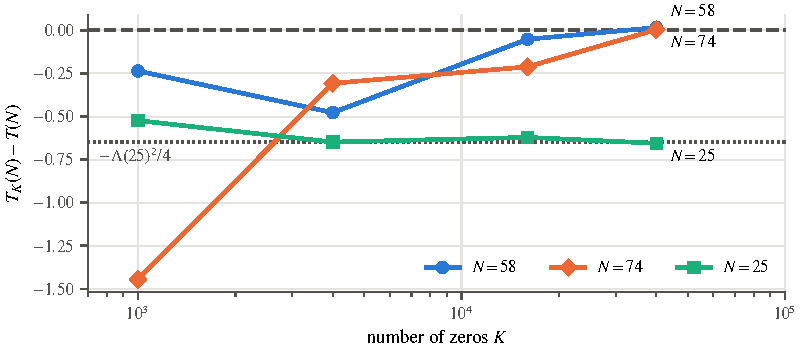
\includegraphics[width=0.85\textwidth]{figs/F3_zeros.pdf}
\caption{$T_K(N)-T(N)$ against the number $K$ of zeros. For $N=58$ and $74$ the
difference tends to $0$ ($+0.016$ and $+0.004$ at $K=4\cdot10^4$); the hypotheses
$T\mp2P^2$ would sit near $\mp14.7$ and $\mp17.2$, outside the frame. For $N=25=5^2$ the
difference settles near $-0.65$ (see the text below Table~\ref{tab:valid}); dotted
line: the level $-\Lambda(25)^2/4$, for reference only.}
\label{fig:zeros}
\end{figure}

\subsection{Fits of \texorpdfstring{$F$}{F}}
Table~\ref{tab:fits} summarises the least-squares fits $F(N)/N=c+\beta P(N)^2/N$.
Figure~\ref{fig:fit} shows the data against the predicted line, and
Figure~\ref{fig:resid} the residual $(F(N)-P(N)^2)/N$, which is constant to within
$10^{-4}$ and shows no $N\log\log N$ signature at values of $N$ with $2N$ highly
composite.

\begin{table}[H]
\centering
\small
\caption{Fits of $F(N)/N$ in the two implementations. Last data row: $2N$ of primorial type (A) and the $N$ with $\rG(2N)/2N>3$ (B), mean $\pm$ s.d.\ of $(F-P^2)/N$.}
\label{tab:fits}
\begin{tabular}{@{}lll@{}}
\toprule
 & A ($1560$ $N$, $[10^6,5\cdot10^6]$) & B ($409$ $N$, $[2.2\cdot10^5,6.0\cdot10^6]$)\\
\midrule
fit $F/N=c+\beta P^2/N$ & $c=-7.351498$, $\beta=0.999933$ & $c=-7.351500$, $\beta=0.999875$\\
s.d.\ of residual & $6.66\cdot10^{-5}$ & $7.55\cdot10^{-5}$\\
$(F-P^2)/N$: mean (s.d.) & $-7.351501$ ($6.67\cdot10^{-5}$) & $-7.351506$ ($7.58\cdot10^{-5}$)\\
$(F-P^2)/N$: range & $[-7.351697,-7.351278]$ & $[-7.351816,-7.351116]$\\
s.d.\ of $(F-kP^2)/N$, $k=0,1,2$ & $6.344\cdot10^{-2}$ ($k=0$) & $5.692\cdot10^{-2}$, $\mathbf{7.581\cdot10^{-5}}$, $5.694\cdot10^{-2}$\\
$\max P^2/N$ & $0.3553$ & $0.3006$\\
$\operatorname{corr}\bigl((F-P^2)/N,\ \rG(2N)/2N\bigr)$ & $-0.0403$ & $0.011$\\
$2N$ highly composite & $60$ $N$: $-7.351498\pm9.98\cdot10^{-5}$ & $83$ $N$: $-7.351504\pm7.42\cdot10^{-5}$\\
\midrule
$-4\log2\pi$ & \multicolumn{2}{c}{$-7.351508$}\\
\bottomrule
\end{tabular}
\end{table}

\begin{figure}[H]
\centering
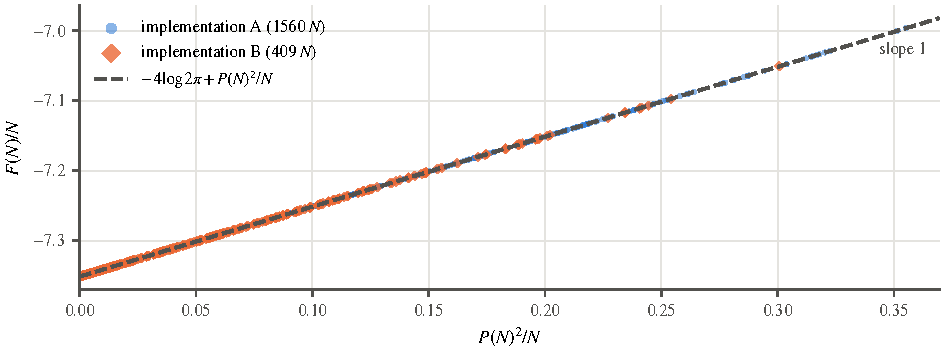
\includegraphics[width=\textwidth]{figs/F1_fit.pdf}
\caption{$F(N)/N$ against $P(N)^2/N$ for the $1969$ computed values of $N$. Dashed line:
slope $1$, intercept $-4\log2\pi$, as predicted by Theorem~\ref{thm:main} and
Remark~\ref{rem:constant}.}
\label{fig:fit}
\end{figure}

\begin{figure}[H]
\centering
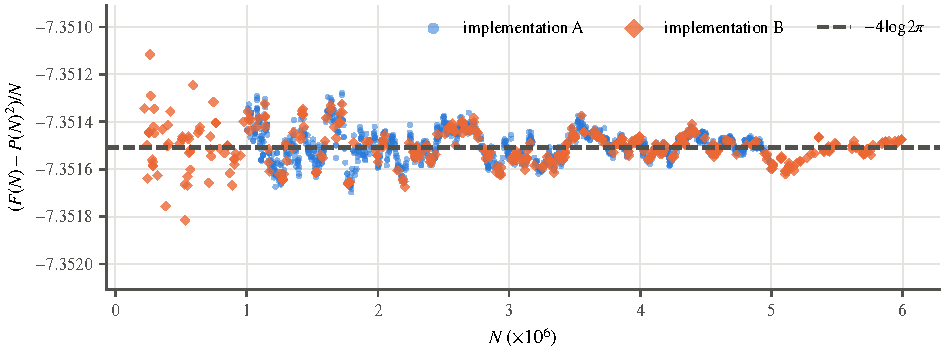
\includegraphics[width=\textwidth]{figs/F2_residual.pdf}
\caption{The residual $(F(N)-P(N)^2)/N$ against $N$, in both implementations. Dashed
line: $-4\log2\pi$.}
\label{fig:resid}
\end{figure}

As an example, at $2N=2012010$ (implementation A), where $\rG(2N)/2N=5.188530$, one has
$(F-P^2)/N=-7.351437$, and the same value at $N\pm1$ ($-7.351437$, $-7.351431$), while
$T(N)/N$ goes from $-2.212$ to $+0.296$ to $+2.810$: the jumps of $\rG$ are carried
entirely by $T$, as Theorem~\ref{thm:C} predicts.

The data show that $F$ contains exactly one copy of $P^2$: $\beta=1.0000\pm10^{-4}$ in
both implementations, and $k=1$ is the only coefficient for which $(F-kP^2)/N$ has
standard deviation of order $10^{-4}$. They do \emph{not} show $F\ne O(N)$, since
$P(N)^2/N\le0.36$ in this range; that is an asymptotic statement, which follows only from
Littlewood's theorem.

%% =====================================================================
\section{The case \texorpdfstring{$k=0$}{k=0}}\label{sec:remarks}
%% =====================================================================

Cantarini notes (\Ca{}, p.~3) that the first part of $T(N)$ is ``what we expect
considering the formula in [BKP] and taking $k=0$''. Brüdern, Kaczorowski and
Perelli~\cite{BKP} prove explicit formulae for the Cesàro--Riesz means of order $k>0$ and
call their formula for $k=0$ purely formal; Theorem~\ref{thm:C} is consistent with this,
since for $k=0$ the term over pairs of zeros must carry the jumps $\rG(n)$ and cannot be
$O(N)$.

%% =====================================================================
\section*{Data availability}
%% =====================================================================
Code and data are available at \url{https://github.com/giovanedms/goldbach-cantarini}
(Zenodo DOI to be assigned).

\section*{Funding}
This research did not receive any specific grant from funding agencies in the public,
commercial, or not-for-profit sectors.

\section*{Declaration of competing interest}
The author declares no competing interests.

\bibliographystyle{amsplain}
\bibliography{refs}

\end{document}
